%%%%%%%%%%%%%%%%%%%%%%%%%%%%%%%%%%%%%%%%%
% Beamer Presentation
% LaTeX Template
% Version 1.0 (10/11/12)
%
% This template has been downloaded from:
% http://www.LaTeXTemplates.com
%
% License:
% CC BY-NC-SA 3.0 (http://creativecommons.org/licenses/by-nc-sa/3.0/)
%
%%%%%%%%%%%%%%%%%%%%%%%%%%%%%%%%%%%%%%%%%

%----------------------------------------------------------------------------------------
%	PACKAGES AND THEMES
%----------------------------------------------------------------------------------------

\documentclass{beamer}

\mode<presentation> {

% The Beamer class comes with a number of default slide themes
% which change the colors and layouts of slides. Below this is a list
% of all the themes, uncomment each in turn to see what they look like.

\usetheme{default}
%\usetheme{AnnArbor}
%\usetheme{Antibes}
%\usetheme{Bergen}
%\usetheme{Berkeley}
%\usetheme{Berlin}
%\usetheme{Boadilla}
%\usetheme{CambridgeUS}
%\usetheme{Copenhagen}
%\usetheme{Darmstadt}
%\usetheme{Dresden}
%\usetheme{Frankfurt}
%\usetheme{Goettingen}
%\usetheme{Hannover}
%\usetheme{Ilmenau}
%\usetheme{JuanLesPins}
%\usetheme{Luebeck}
%\usetheme{Madrid}
%\usetheme{Malmoe}
%\usetheme{Marburg}
%\usetheme{Montpellier}
%\usetheme{PaloAlto}
%\usetheme{Pittsburgh}
%\usetheme{Rochester}
%\usetheme{Singapore}
%\usetheme{Szeged}
%\usetheme{Warsaw}

% As well as themes, the Beamer class has a number of color themes
% for any slide theme. Uncomment each of these in turn to see how it
% changes the colors of your current slide theme.

%\usecolortheme{albatross}
%\usecolortheme{beaver}
%\usecolortheme{beetle}
%\usecolortheme{crane}
%\usecolortheme{dolphin}
%\usecolortheme{dove}
%\usecolortheme{fly}
%\usecolortheme{lily}
%\usecolortheme{orchid}
%\usecolortheme{rose}
%\usecolortheme{seagull}
%\usecolortheme{seahorse}
%\usecolortheme{whale}
%\usecolortheme{wolverine}

%\setbeamertemplate{footline} % To remove the footer line in all slides uncomment this line
%\setbeamertemplate{footline}[page number] % To replace the footer line in all slides with a simple slide count uncomment this line

%\setbeamertemplate{navigation symbols}{} % To remove the navigation symbols from the bottom of all slides uncomment this line
}

\usepackage{graphicx} % Allows including images
\usepackage{booktabs} % Allows the use of \toprule, \midrule and \bottomrule in tables

%----------------------------------------------------------------------------------------
%	TITLE PAGE
%----------------------------------------------------------------------------------------

\title[Short title]{Suosittelijajärjestelmän rakentaminen Apache Sparkilla} % The short title appears at the bottom of every slide, the full title is only on the title page

\author{Jonne Pihlanen} % Your name
\institute[TUT] % Your institution as it will appear on the bottom of every slide, may be shorthand to save space
{
Tampereen Teknillinen Yliopisto \\ % Your institution for the title page
\medskip
\textit{jonne.pihlanen@student.tut.fi} % Your email address
}
\date{\today} % Date, can be changed to a custom date

\begin{document}

\begin{frame}
\titlepage % Print the title page as the first slide
\end{frame}

\begin{frame}
\frametitle{Sisältö} % Table of contents slide, comment this block out to remove it
\tableofcontents % Throughout your presentation, if you choose to use \section{} and \subsection{} commands, these will automatically be printed on this slide as an overview of your presentation
\end{frame}

%----------------------------------------------------------------------------------------
%	PRESENTATION SLIDES
%----------------------------------------------------------------------------------------

\section{Tavoitteet}

\begin{frame}
\frametitle{Tavoitteet}

Elokuvien suosittelua Apache Sparkin avulla.
Koska työ tehtiin vain omaksi iloksi, ajatuksena oli hyödyn maksimointi ja tavoitteeksi valittiin: uuden ohjelmointikielen opettelu, pilvipalveluun tutustuminen sekä Spark-ohjelmistokehykseen tutustuminen.
Akateeminen osuus hoidettiin etsimällä tutkimuspaperi, johon perustin oman mallini opetuksen.

\end{frame}

%------------------------------------------------

%------------------------------------------------
\section{Teoria}
%------------------------------------------------

\begin{frame}
\frametitle{Suosittelijajärjestelmät}

\begin{itemize}
	\item Suosittelijajärjestelmät ovat joukko tekniikoita ja ohjelmistoja, jotka tarjovat suosituksia mahdollisesti hyödyllisistä tuotteista.
	\item Tässä työssä keskitytään yhteisösuodattamiseen (collaborative filtering): jos käyttäjät pitivät samankaltaisista tuotteista aikaisemmin, he luultavasti pitävät samoja tuotteita ostaneiden henkilöiden suosituksia merkityksellisinä.
	\item Muistipohjainen (Käyttäjäpohjainen, Tuotepohjainen)
	\item Mallipohjainen (ALS)
\end{itemize}

\end{frame}

%------------------------------------------------

\begin{frame}
\frametitle{Alternating Least Squares (ALS)}

\begin{itemize}
	\item Spark ALS yrittää arvata arvostelumatriisin $A$ kahden tekijämatriisin, $X$ ja $Y$, tulona.
	\item Perinteinen lähestymistapa on iteratiivinen.
	\item Jokaisen iteraation aikana toista tekijämatriisia pidetään vakiona ja toinen ratkaistaan käyttäen MSE-algoritmia.
	\item Juuri ratkaistua tekijämatriisia pidetään vuorostaan vakiona kun ratkaistaan toista tekijämatriisia.
	\item Löydetty ratkaisu takaa minimaalisen MSE:n, jokaisella askeleella ratkaisu voi joko pienentyä tai pysyä samana, mutta ei kasvaa.
	\item Algoritmi vaihtelee (\textbf{alternates}) näiden kahden askeleen välillä konvergenssiin asti.
	\item ALS on siis kaksivaiheinen iteratiivinen optimointiprosessi.
\end{itemize}

\end{frame}

%------------------------------------------------

\begin{frame}
\frametitle{Root Mean Square Error (RMSE)}

Työn mallin opetusvirheen arviointiin käytettiin RMSE -metriikkaa.

\begin{itemize}
	\item kenties suosituin ennustettujen arvosteluiden tarkkuuden evaluointiin käytetty metriikka.
	\item RMSE:n tuntemiseksi tulee tuntea ensin MSE (Mean Square Error).
	\item MSE on virheiden neliöiden keskiarvo ja se voidaan laskea neliöimällä jokaisen havainnon virhe ja laskemalla virheiden neliöiden keskiarvo.
	\item RMSE voidaan puolestaan laskea ottamalla neliöjuuri MSE:stä.
\end{itemize}

Pienimmän RMSE:n omaavan mallin voidaan sanoa sovittuvan parhaiten opetusdataan.

\end{frame}

%------------------------------------------------

%------------------------------------------------
\section{Teknologiat}
%------------------------------------------------

\begin{frame}
\frametitle{Scala}

\begin{itemize}
	\item Scala on moniparadigmainen ohjelmointikieli, joka tukee sekä olio- että funktionaalista ohjelmointia.
	\item Muuttumattomat tietorakenteet ja funktiot ensimmäisen luokan kansalaisina.
	\item Luokat ja oliot, kapselointi, perintä, moniperintä.
	\item Scala on staattisesti tyypitetty kieli ja sillä kirjoitetut ohjelmat käännetään Scala-kääntäjää käyttäen.
	\item Scala on JVM-kieli, joten Scala käännetään Java-tavukoodiksi, jota voidaan ajaa missä tahansa Java-virtuaalikoneessa.
\end{itemize}

\end{frame}

%------------------------------------------------

\begin{frame}
\frametitle{Apache Spark}

\begin{itemize}
	\item Yleispätevä analytiikkasovelluskehys
	\item (RDD), Dataset, DataFrame, MLlib
	\item Nopeus + käyttäjäystävällisyys
	\item muistissa tapahtuva prosessointi
	\item Parhaimmillaan hurjasti nopeampi kuin Hadoop: Ei rajoitettu kahteen steppiin $=>$ Spark voi suoriutua yhdellä monitasoisella ajolla kun taas MapReduce tekee aina kaksi ennalta määrättyä toimea (map ja reduce)
	\item Kirjoitettu Scala-ohjelmointikielellä ja Sparkia voi kirjoittaa Scalalla, mutta lisäksi esimerkiksi Pythonilla, R:llä ja jopa Kotlinilla.
\end{itemize}

\end{frame}

%------------------------------------------------

\begin{frame}
\frametitle{Amazon Web Services (AWS)}

Amazonin tarjoama kokoelma pilvilaskentaan (cloud computing) tarkoitettuja tai sitä avustavia palveluita.
Työssä käytettiin varsinaisesti kahta AWS:n palvelua: Elastic Map Reducea (EMR) ja Simple Storage Serviceä (S3).

~

\begin{itemize}
	\item [EMR] Hallittu klusterialusta esimerkiksi Apache Sparkin ajamiseen
	\item [S3] Tietovarasto
\end{itemize}

\end{frame}

%-----------------------------------------------------------

%-----------------------------------------------------------
\section{Toteutus}
%-----------------------------------------------------------

\begin{frame}
\frametitle{Toteutus}

\begin{itemize}
	\item EMR-konfigurointi
	\item Opetusdata
	\item Projektin rakenne
	\item Opetusdatan lataaminen
	\item Mallin opettaminen
	\item Opetusvirheen evaluointi
	\item Ennustaminen
\end{itemize}

\end{frame}

%------------------------------------------------

%------------------------------------------------
\section{Tulokset}
%------------------------------------------------

\begin{frame}
\frametitle{Sisääntulot}

\begin{tabular}{lll}
	Tunniste & Nimi & Arvostelu \\ \hline
	112897 & The Expendables 3 (2014) & 4.0 \\
	116887 & Exodus: Gods and Kings (2014) & 4.0 \\
	117529 & Jurassic World (2015) & 4.0 \\
	128520 & The Wedding Ringer (2015) & 4.5 \\
	122882 & Mad Max: Fury Road (2015) & 4.0 \\
	131013 & Get Hard (2015) & 4.0 \\
	132796 & San Andreas (2015) & 3.0 \\
	136305 & Sharknado 3: Oh Hell No! (2015) & 1.0 \\
	136598 & Vacation (2015) & 4.0 \\
	137595 & Magic Mike XXL (2015) & 1.0 \\
	138208 & The Walk (2015) & 2.0 \\
	140523 & The Visit (2015) & 3.5 \\
	146656 & Creed (2015) & 4.0 \\
	148626 & The Big Short (2015) & 4.5 \\
	149532 & Marco Polo: One Hundred Eyes (2015) & 4.5 \\
\end{tabular}

\end{frame}

%------------------------------------------------

\begin{frame}
\frametitle{Tulokset}

\begin{itemize}
	\item \textbf{The War at Home (1979)} Drama
	\item \textbf{Pearl Jam: Immagine in Cornice (2007)} Documentary, Music
	\item \textbf{Octopus (2000)} Adventure, Horror
	\item \textbf{My Brother Tom (2001)} Drama
	\item \textbf{Return to the 36th Chamber (1980)} Action, Comedy
	\item \textbf{Bob Funk (2009)} Comedy
	\item \textbf{Hamoun (1990)} Drama
	\item \textbf{Notebook (2006)} Drama, Musical, Romance
	\item \textbf{Patton Oswalt: My Weakness Is Strong (2009)} Documentary, Comedy
	\item \textbf{Deathstalker II (1987)} Adventure, Comedy, Fantasy
\end{itemize}

\end{frame}

%------------------------------------------------

%------------------------------------------------
\section{Johtopäätökset}
%------------------------------------------------

\begin{frame}
\frametitle{Johtopäätökset}

Tulokset eivät olleet kovin lupaavia, enemmän omia arvosteluja ja vieläkin isommalla MovieLens-datasetillä kouluttaminen voisi kuvitella auttavan.

\end{frame}

%------------------------------------------------

\begin{frame}
\frametitle{Loppukevennys}

\begin{figure}[h]
	\centering
	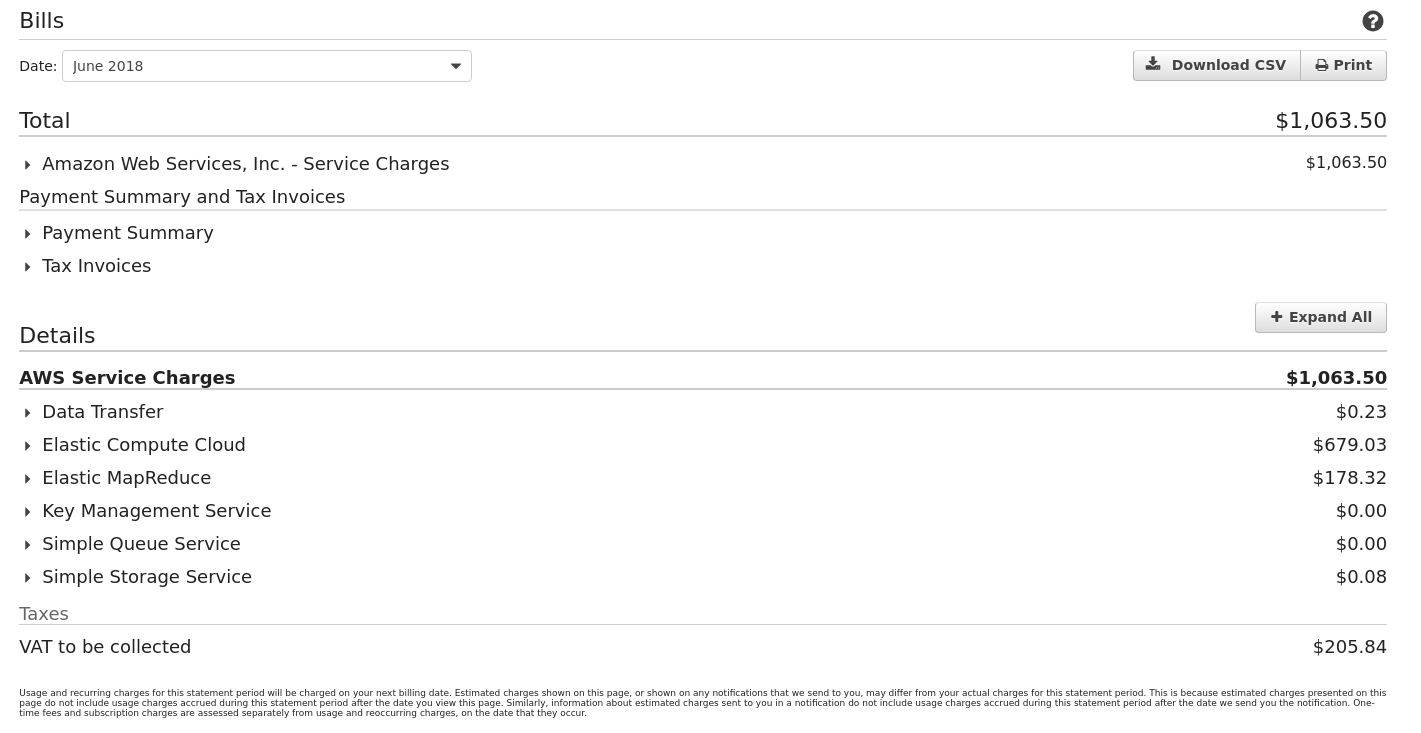
\includegraphics[scale=0.2]{../images/aws_bill}
\end{figure}

\end{frame}

%------------------------------------------------

\begin{frame}

Kiitos! Kysymyksiä?

\end{frame}

%------------------------------------------------

\end{document} 